\documentclass{article}
\usepackage{graphicx}
\usepackage{listings}
\usepackage{color}
\definecolor{dkgreen}{rgb}{0,0.6,0}
\definecolor{gray}{rgb}{0.5,0.5,0.5}
\definecolor{mauve}{rgb}{0.58,0,0.82}

\lstset{frame=tb,
  language=c,
  aboveskip=3mm,
  belowskip=3mm,
  showstringspaces=false,
  columns=flexible,
  basicstyle={\small\ttfamily},
  numbers=none,
  numberstyle=\tiny\color{gray},
  keywordstyle=\color{blue},
  commentstyle=\color{dkgreen},
  stringstyle=\color{mauve},
  breaklines=true,
  breakatwhitespace=true,
  tabsize=3
}
\author{Group 9}
\title{TCP/IP file transfer}
\begin{document}
\maketitle
\section{Protocol Design}
\subsection{Figure}
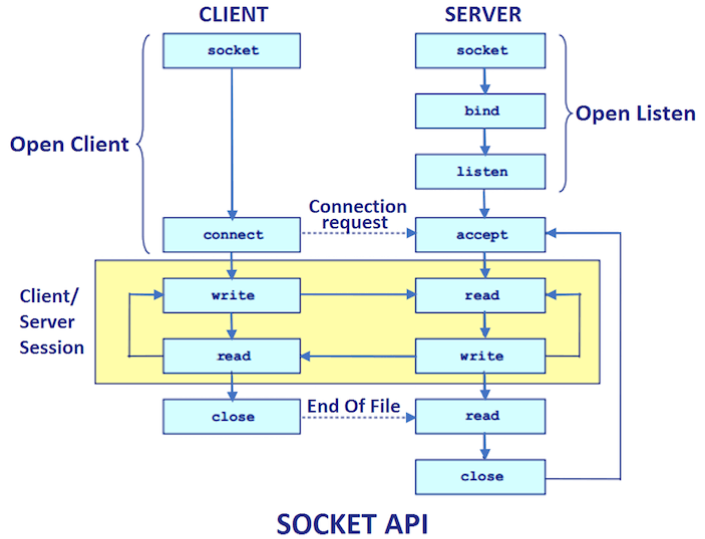
\includegraphics{Capture.PNG}
\newpage
\section{System Organizing}
{We start create 2 socket both for server and client}
\subsection{Open Session}
\begin{itemize}
    \item The server socket will be bound to port 4444 after created 
    \item The server socket then listening to any message/data received
\end{itemize}
\subsection{End open listen of server}
\begin{itemize}
    \item After getting the server socket to listening, the client socket will try to connect to the server
\end{itemize}
\subsection{End open client socket}
\begin{itemize}
    \item In client/Server session, both client and server sending each other message alternatively until ones decided to close.
\end{itemize}
\newpage
\section{Code Implementation}
\subsection{Client}
\begin{lstlisting}
#include <stdio.h>
#include <stdlib.h>
#include <string.h>
#include <sys/socket.h>
#include <sys/types.h>
#include <netinet/in.h>
#include <arpa/inet.h>
 
#define PORT 4444
int main(){
  
   int clientSocket;
   struct sockaddr_in serverAddr;
   char buffer[1024];
     // socket create and verification
   clientSocket = socket(PF_INET, SOCK_STREAM, 0);
   printf("[+]Client Socket Created Sucessfully.\n");
   memset(&serverAddr, '\0', sizeof(serverAddr));
   serverAddr.sin_family = AF_INET;
   serverAddr.sin_port = htons(PORT);
   serverAddr.sin_addr.s_addr = inet_addr("127.0.0.1");
   // Server is ready to listen and verification
   connect(clientSocket, (struct sockaddr*)&serverAddr, sizeof(serverAddr));
   printf("[+]Connected to Server.\n");
   // Receiver from the sever receiver messeger from sever
   recv(clientSocket, buffer, 1024, 0);
   printf("[+]Data Recv from sever: %s\n", buffer);
   strcpy(buffer, "hillo");
   send(clientSocket, buffer, strlen(buffer), 0);
   printf("[+]Closing the connection.\n");
   return 0;
}
\end{lstlisting}
Implementing
\begin{lstlisting}
hung8585@Hung8585s-MacBook ~ % cd "/Users/hung8585/Downloads/TCP-file_transfer/" && gcc TCP-client.c -o TCP-client && "/Users/hung8585/Downloads/TCP-file_transfer/"TCP-client

[+]Client Socket Created Sucessfully.
[+]Connected to Server.
[+]Data Recv from sever: hello
[+]Closing the connection.
\end{lstlisting}
\subsection{Server}
\begin{lstlisting}
#include <stdio.h>
#include <stdlib.h>
#include <string.h>
#include <sys/socket.h>
#include <sys/types.h>
#include <netinet/in.h>
#include <arpa/inet.h>
 
#define PORT 4444
 
int main(){
 
   int sockfd;
   struct sockaddr_in serverAddr;
 
   int newSocket;
   struct sockaddr_in newAddr;
 
   socklen_t addr_size;
   char buffer[1024];
    // socket create and varification
   sockfd = socket(AF_INET, SOCK_STREAM, 0);
   printf("[+]Server Socket Created Sucessfully.\n");
   memset(&serverAddr, '\0', sizeof(serverAddr));
       // assign IP, PORT
   serverAddr.sin_family = AF_INET;
   serverAddr.sin_port = htons(PORT);
   serverAddr.sin_addr.s_addr = inet_addr("127.0.0.1");
      // Binding newly created socket to given IP and verification
   bind(sockfd, (struct sockaddr*)&serverAddr, sizeof(serverAddr));
   printf("[+]Bind to Port number %d.\n", 4444);
     // Server is ready to listen and verificatio
   listen(sockfd, 5);
   printf("[+]Listening...\n");
 
   newSocket = accept(sockfd, (struct sockaddr*)&newAddr, &addr_size);
      // Send the messeger to client and receiver messeger from client
   strcpy(buffer, "hello");
   send(newSocket, buffer, strlen(buffer), 0);
   recv(newSocket, buffer, 1024, 0);
   printf("[+]Data Recv from client: %s\n", buffer);
   printf("[+]Closing the connection.\n");
   return 0;
}
\end{lstlisting}
\newpage
Implementing
\begin{lstlisting}
[Running] cd "/Users/hung8585/Downloads/TCP-file_transfer/" && gcc TCP-sever.c -o TCP-sever && "/Users/hung8585/Downloads/TCP-file_transfer/"TCP-sever
[+]Server Socket Created Sucessfully.
[+]Bind to Port number 4444.
[+]Listening...
[+]Data Recv from client: hillo
[+]Closing the connection.

\end{lstlisting}
\section{Group participation}
\begin{itemize}
\item Nguyen Trung Dung - BI8029 : Complete and implement the code
\item Ngruyen Trong Son - BI8153: Protocol Explanation
\item Nguyen Khanh Nam - BI8122 : System Explanation
\item Pham Viet Minh Duc BI8045 - : Draw Figure
\item Do Anh Tu - BI8157: Checking and smoothing 
\item Do Thi Minh Ngoc - BI8129: Complete Report
\end{itemize}

\end{document}